\chapter{SRAM PUF}\label{sec:sram_puf}

\gls{sram} \gls{puf} is based on a random startup behaviour of individual \gls{sram} cells. It was first proposed by~\cite{Guajardo2007} in 2007.

In a \gls{cmos} implementation (which is used to create 99\% of integrated circuits as of 2011\cite{Voinigescu2013}) a \gls{sram} cell is usually made up of two cross-coupled inverters. The inverters reinforce each other of their state, thus creating a bistable circuit---a circuit with only two stable states. This enables the cell to save exactly one logical bit. Each inverter is implemented using two transistors and additional two transistors are used to enable read and write operations. This means that storage of a single bit costs six transistors in hardware.\cite{Maes2010}

The logical diagram of a \gls{sram} cell containing the two inverters is illustrated in Figure~\ref{fig:sram_cell_logic} and a diagram with the transistor layout of the cell is shown in Figure~\ref{fig:sram_cell_cmos}.

\begin{figure}[h!]
    \centering
    \captionsetup{justification=centering,margin=0.5cm}
    \begin{subfigure}[c]{0.5\textwidth}
        \centering
        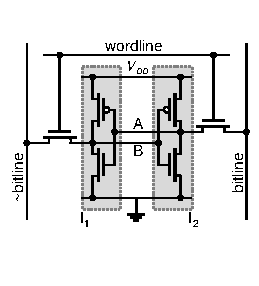
\includegraphics[width=0.85\linewidth]{images/transistor_sram_cell.pdf}
        \caption{A CMOS diagram of a SRAM cell.}
        \label{fig:sram_cell_cmos}
    \end{subfigure}%
    \begin{subfigure}[c]{0.5\textwidth}
        \centering
        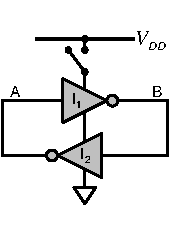
\includegraphics[width=0.6728\linewidth]{images/logic_sram_cell.pdf}
        \caption{A logic circuit diagram of a SRAM cell.}
        \label{fig:sram_cell_logic}
    \end{subfigure}
    \caption[CMOS and logic circuit diagrams of a SRAM cell.]{CMOS and logic circuit diagrams of a SRAM cell.\cite{Maes2012}}
    \label{fig:sram_cell}
\end{figure}

The principle of a \gls{sram} \gls{puf} is based on the power-up values of the memory cells. The memory cells are volatile---when power is lost, the data disappears from memory. After startup, each cell has to initialize to either a `1' or a `0' state. Which state the cell stabilizes on is dependent on a relative strength\footnote{strength here means the properties of the underlying \gls{mosfet} transistors (such as delay)} of the two inverters. Since the inverters are designed identically, their strength is determined by random process variations during manufacturing.\cite{Maes2010}

For each cell independently, the two following cases can happen:

\begin{enumerate}
    \item One of the inverters has far greater strength than the other. The cell has a significant preference for one initial state. Meaning it will either be in the `0' or the `1' state most of the time after power-up. This case is crucial for the \gls{puf} construction.
    \item By chance, strengths of the two inverters are nearly identical. The resulting initial state depends on random noise in the circuit. This is the source of unreliability of the \gls{puf}.
\end{enumerate}

During fabrication, each cell acquires its specific properties and thus its startup state stability according to the cases mentioned above. However, stability is not a discrete property. One cell can be less stable than some other. An illustration of this can be seen in Figure~\ref{fig:sram_puf_stability}.

\begin{figure}[ht!]
    \centering
    \captionsetup{justification=justified,margin=0.5cm}
    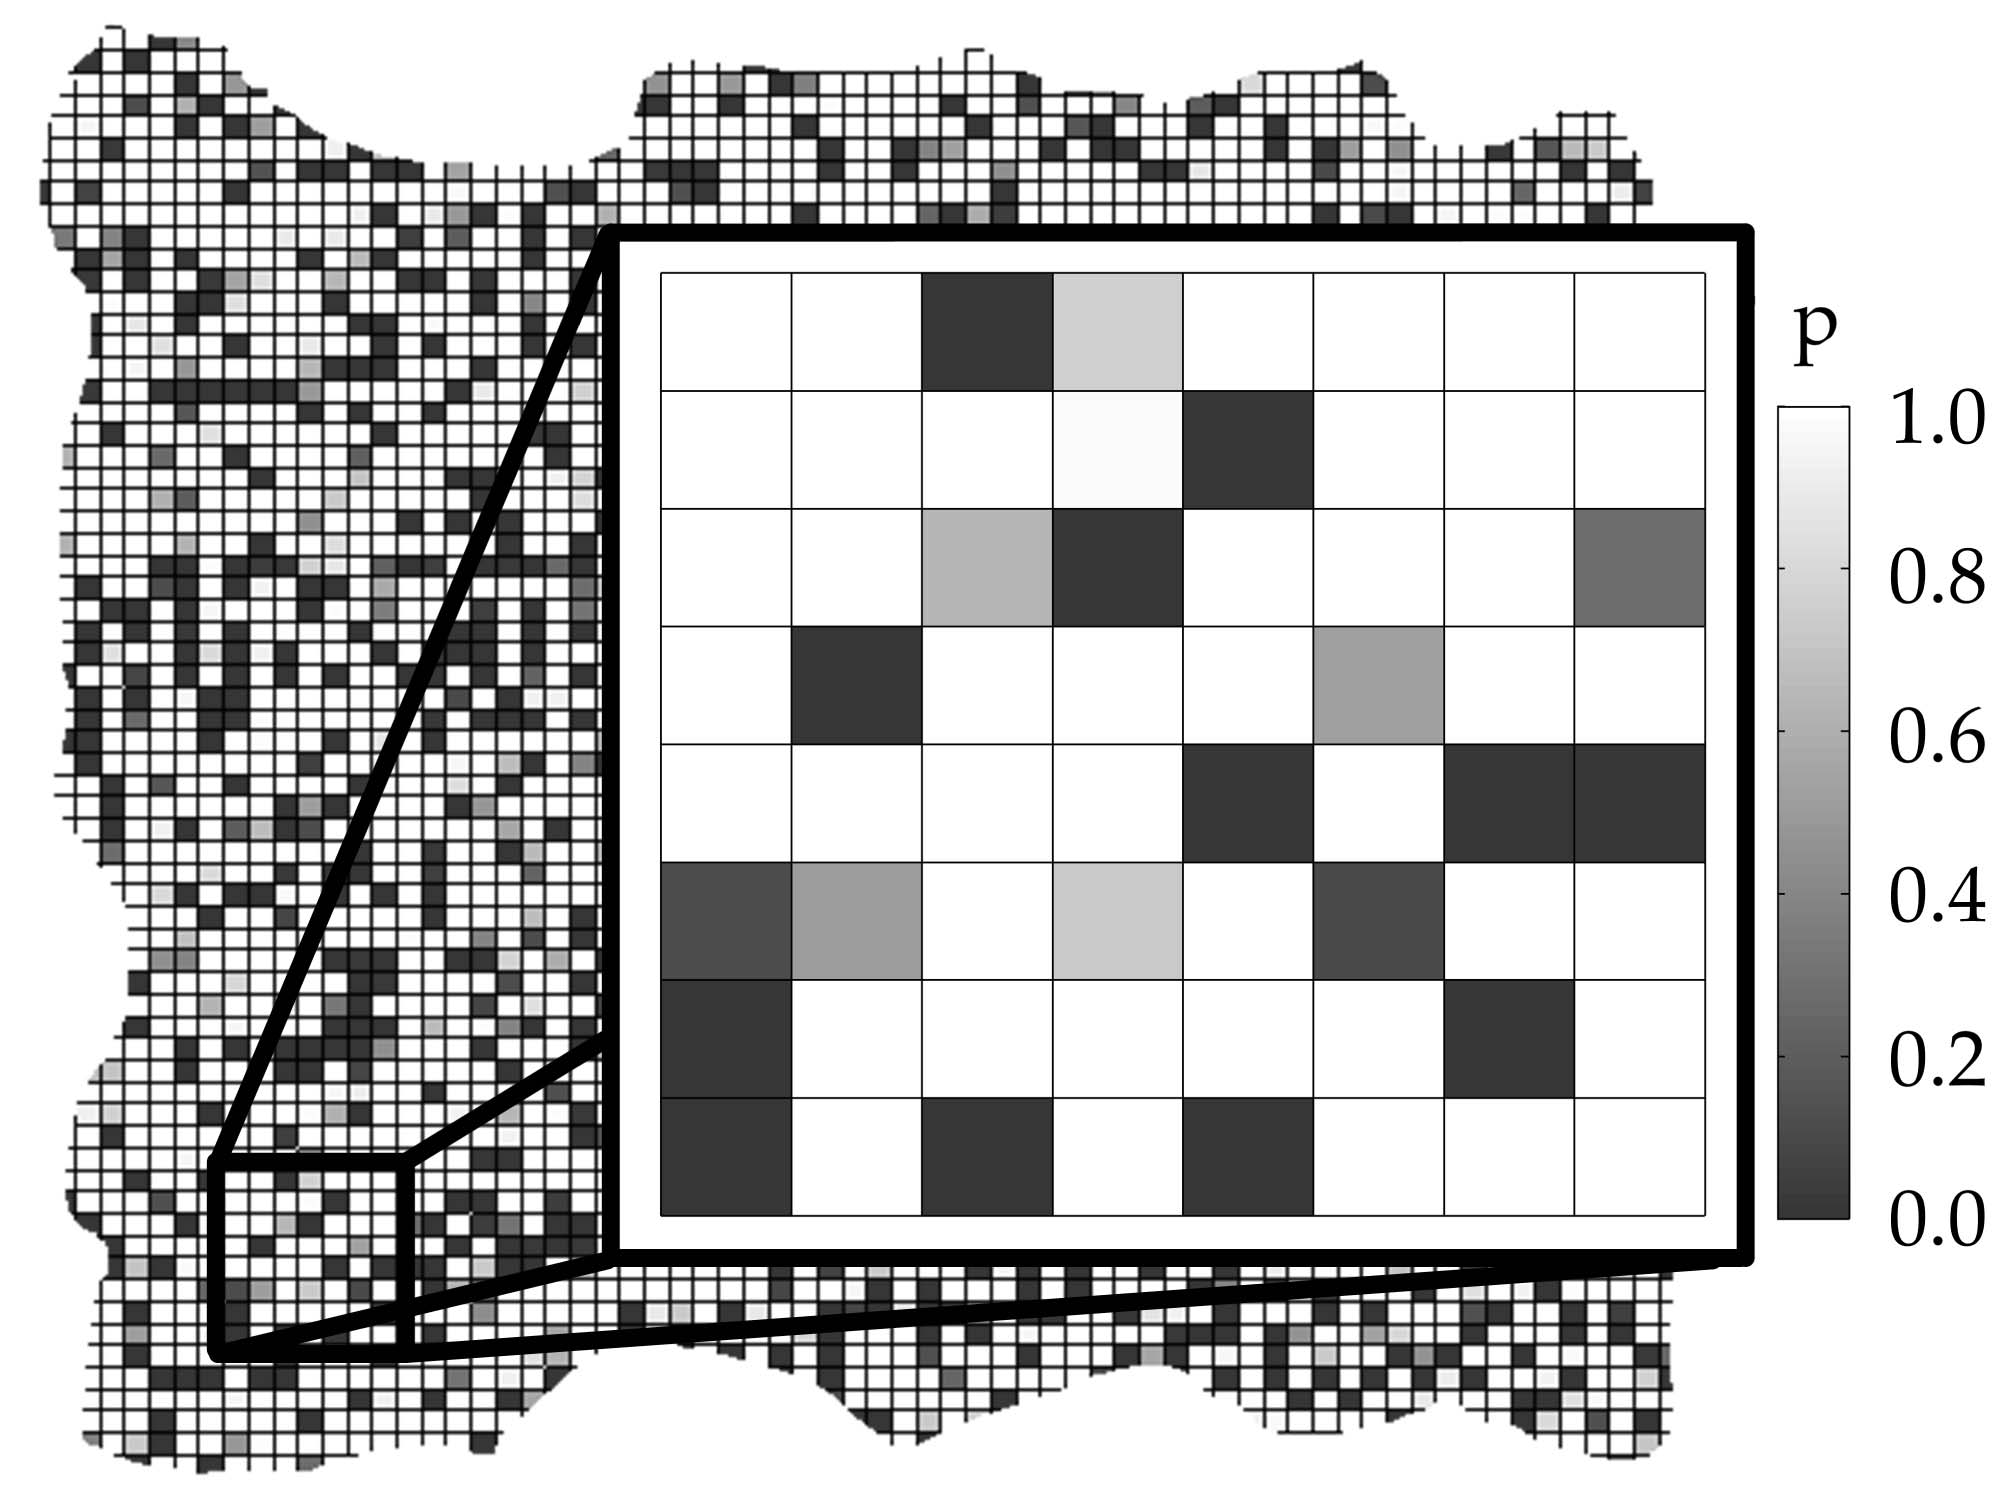
\includegraphics[width=0.5\textwidth]{images/sram_puf_stability.jpg}
    \caption[Illustration of SRAM cell stability.]{Illustration of SRAM cell stability. A small area of SRAM cells is shown. The lightness of each cell indicates the probability that the cell's startup state will be `1'. Note that most of the cells are either nearly black or nearly white. Meaning they are stable and their preferred state is `0` or `1` respectively.~\cite{Holcomb2009}.}
    \label{fig:sram_puf_stability}
\end{figure}

It turns out, that the process variations are significant enough that most \gls{sram} cells tend to be stable. This enables the startup values of memory to be used as \gls{puf} responses. Challenge can be interpreted as a concrete address in memory. The response is then read from this address.\cite{Maes2013}

For the construction of a \gls{sram} \gls{puf}, stable cells are important. The unstable ones can be considered harmful as they decrease reliability. However, thanks to their unknown initial state which is determined randomly after every startup, they are useful for the construction of \glspl{trng}.\cite{Holcomb2009}

A huge advantage of \gls{sram} \glspl{puf} is, that \gls{sram} memory is usually already present in chips. If the device possesses a suitable mechanism of power state control of its memory (the ability to turn off blocks of memory, power-saving states that turn off memory), no additional hardware is needed. Therefore this type of \gls{puf} could potentially be implemented in devices that were not designed to contain a \gls{puf} at all.

Data remanence time of \gls{sram} memory needs to be taken into account as well. The memory cell remembers its state even for a short period of time after power is lost. If power is turned on again before this time, the saved data can still be found in memory. The remanence time is greatly affected by temperature. Lower temperature results in longer retention time. This effect can be observed on the ESP32 \gls{sram} in Sections~\ref{sec:deep_sleep_analysis} and~\ref{sec:rtc_analysis}.

The \gls{puf} implementation must guarantee that the memory has been unpowered long enough. Otherwise, the startup memory values used as a \gls{puf} response can be altered by a potential attacker and can be for example used to manipulate the reconstructed cryptographic key.\cite{Nikolaos2018}

\section{SRAM PUF and its properties}\label{sec:srampuf_properties}

\glspl{puf} constructions can be characterized by several properties. They have been discussed in Section~\ref{sec:properties}. However, not every \gls{puf} needs to exhibit all of them. Therefore a discussion about what particular properties a \gls{sram} \gls{puf} meets is provided according to \cite{Maes2013}. The summary of properties of \gls{sram} \gls{puf} can be found in Table~\ref{table:sram_puf_properties}.

\begin{table}[ht!]
\centering
\begin{tabular}{l c} 
    \textbf{Property} & \textbf{\gls{sram} \gls{puf}} \\
     \toprule
    Constructibility & yes\\ 
    Evaluability & yes\\
    Reproducibility & yes\\
    Uniqueness & yes\\
    Identifiability & yes\\ 
    Physical Unclonability & yes\\
    Unpredictability & yes\\
    Mathematical unclonability & no\\
    True unclonability & no\\
    One-Wayness & no\\
    Tamper evidence & probably no\\
     \bottomrule
    \end{tabular}
    \captionsetup{justification=centering,margin=0.5cm}
    \caption{Summarization of properties of SRAM PUF.}
    \label{table:sram_puf_properties}
\end{table}


\begin{description}
    \item[Constructibility:] \hfill \\
        Since known implementations of \gls{sram} \gls{puf} exist (and one is provided in this thesis), it is definitely constructible. Furthermore, the effort needed to construct the \gls{puf} is low compared to the other implementations---\gls{sram} memory is usually already present in chips and no additional hardware is needed.
    \item[Evaluability:] \hfill \\
        \gls{sram} \gls{puf} is evaluable because it is possible to read the startup values of the \gls{sram} cells which are interpreted as the response. However, the effort to obtain the response can be rather high since the memory needs to be read fresh after power up (before the response is overwritten by other data). Depending on the device used and its capabilities, this could potentially require procedures that take a long time (for example rebooting the device or using a power-saving state to turn off the \gls{sram} memory). Additional hardware could mitigate this problem, increasing manufacturing costs.
    \item[Reproducibility:] \hfill \\
        The \gls{sram} \gls{puf} possesses the reproducibility property because memory cells have a preference for some initial state. This preference is imprinted on the cell at the time of manufacturing and does not change much afterwards (however, \gls{sram} aging effect can alter the preference of a cell over time and this is discussed later in this section). % TODO fakt jsem napsal neco o sram aging?
    \item[Uniqueness:] \hfill \\
        \gls{sram} \glspl{puf} are unique, as each memory cell creates its preference for some initial state during manufacturing independently. For this reason, the resulting \gls{puf} responses from different devices should not be similar.
    \item[Identifiability:] \hfill \\
        As identifiability is the combination of reproducibility and uniqueness, both of which are already met, the \gls{sram} \gls{puf} is identifiable as well. This means that the intra-\gls{hd} and inter-\gls{hd} distributions are sufficiently separated and the responses can be used to identify devices.
    \item[Physical unclonability:] \hfill \\
        The source of randomness of \gls{sram} \glspl{puf} is the physical variation of individual transistors that implement the memory cells. These variations take place on a micro/nano scale and are technically infeasible to control fully. Even the manufacturer is unable to create two \gls{sram} memory instances with similar cell startup state preferences. Thus this construction is considered physically unclonable.
    \item[Unpredictability:] \hfill \\
        Unpredictability assumes, that given a limited set of challenge-response pairs, no prediction algorithm can be designed for future challenges. Responses are interpreted as memory addresses and each cell should acquire its preference for some initial state independently. Therefore the knowledge of a challenge-response pair does not reveal any information about other pairs. For this reason, \gls{sram} \glspl{puf} are unpredictable. % TODO mozna napsat neco k PUFum s jednim challengem?
    \item[Mathematical unclonability:] \hfill \\
        Mathematical unclonability is a stronger model of unpredictability. It assumes having access to as many challenge-response pairs as can be stored. Since \gls{sram} \glspl{puf} have only a limited number of those pairs (only one in the extreme case), a simple lookup table with all the possible pairs can be constructed easily. Thus, the property of mathematical unclonability is not met.
    \item[True unclonability:] \hfill \\
        A \gls{puf} is truly unclonable if it is physically and mathematically unclonable. Therefore, by definition, \gls{sram} \gls{puf} is not truly unclonable since it is not mathematically unclonable.
    \item[One-wayness:] \hfill \\
        One-wayness (similar to mathematical unclonability) requires the \gls{puf} to have a sufficiently large challenge and response sets. Because \gls{sram} \glspl{puf} are weak, they are not one-way.
    \item[Tamper evidence:] \hfill \\
        Not enough research has been conducted to declare whether \gls{sram} \glspl{puf} are tamper evident or not\cite{Maes2012}. However, it has been shown that it is possible to strip the device of most unrelated silicon without changing the \gls{puf} response significantly\cite{Helfmaier2013}. Additionally,~\cite{Nedospasov2013} showed that it is possible to extract full \gls{puf} responses from AVR microcontrollers\footnote{the experiment was conducted on an ATMega328P and an ATXMega128A1 models} by disabling the logic core and using a semi-invasive laser probing technique to read the startup memory values.
\end{description}


\section{Stable response extraction}
% je tahle sekce OK???

Since \gls{sram} \glspl{puf} are weak, they are usually used for key generation. The resulting key must be the same every time it is reconstructed. Therefore, stability of the response needs to be guaranteed. Several methods that increase stability exist: \gls{tmv}, \gls{ecc}, direct bit preselection and indirect bit preselection.\cite{Shifman2018}

\subsubsection*{Temporal majority voting}

 \gls{tmv} samples the \gls{puf} response multiple times and the resulting response is based on bitwise majority vote of the samples. This increases the time it takes to obtain the response significantly. Additionally, if a cell is very unstable, the majority vote for it could be very close and thus not stable.

\subsubsection*{Error correction codes}

 \gls{ecc} correct the errors in the response, thus increasing stability. However, they need to store helper data in non-volatile memory to function, decrease response length and have computational overhead. A simple repetition \gls{ecc} is used in the \gls{sram} \gls{puf} implementation in this thesis and details will be discussed in Section~\ref{sec:ecc}.

\subsubsection*{Direct bit preselection}

Stable bit preselection methods try to indicate which bits are stable and they create a mask of stable bits. This mask is saved to a non-volatile memory of the device and is later used to ignore the unstable bits during response extraction.

In direct preselection, the \gls{puf} response is first measured multiple times. Stable bits are identified based on their average startup value over multiple measurements. To identify more stable bits, measurements can be made across different operating temperatures and supply voltages. However, this is a very time consuming technique. An example of average startup \gls{sram} cells can be seen in Figure~\ref{fig:bit_stability_mask}.

\begin{figure}[ht!]
    \centering
    \captionsetup{justification=justified,margin=0.5cm}
    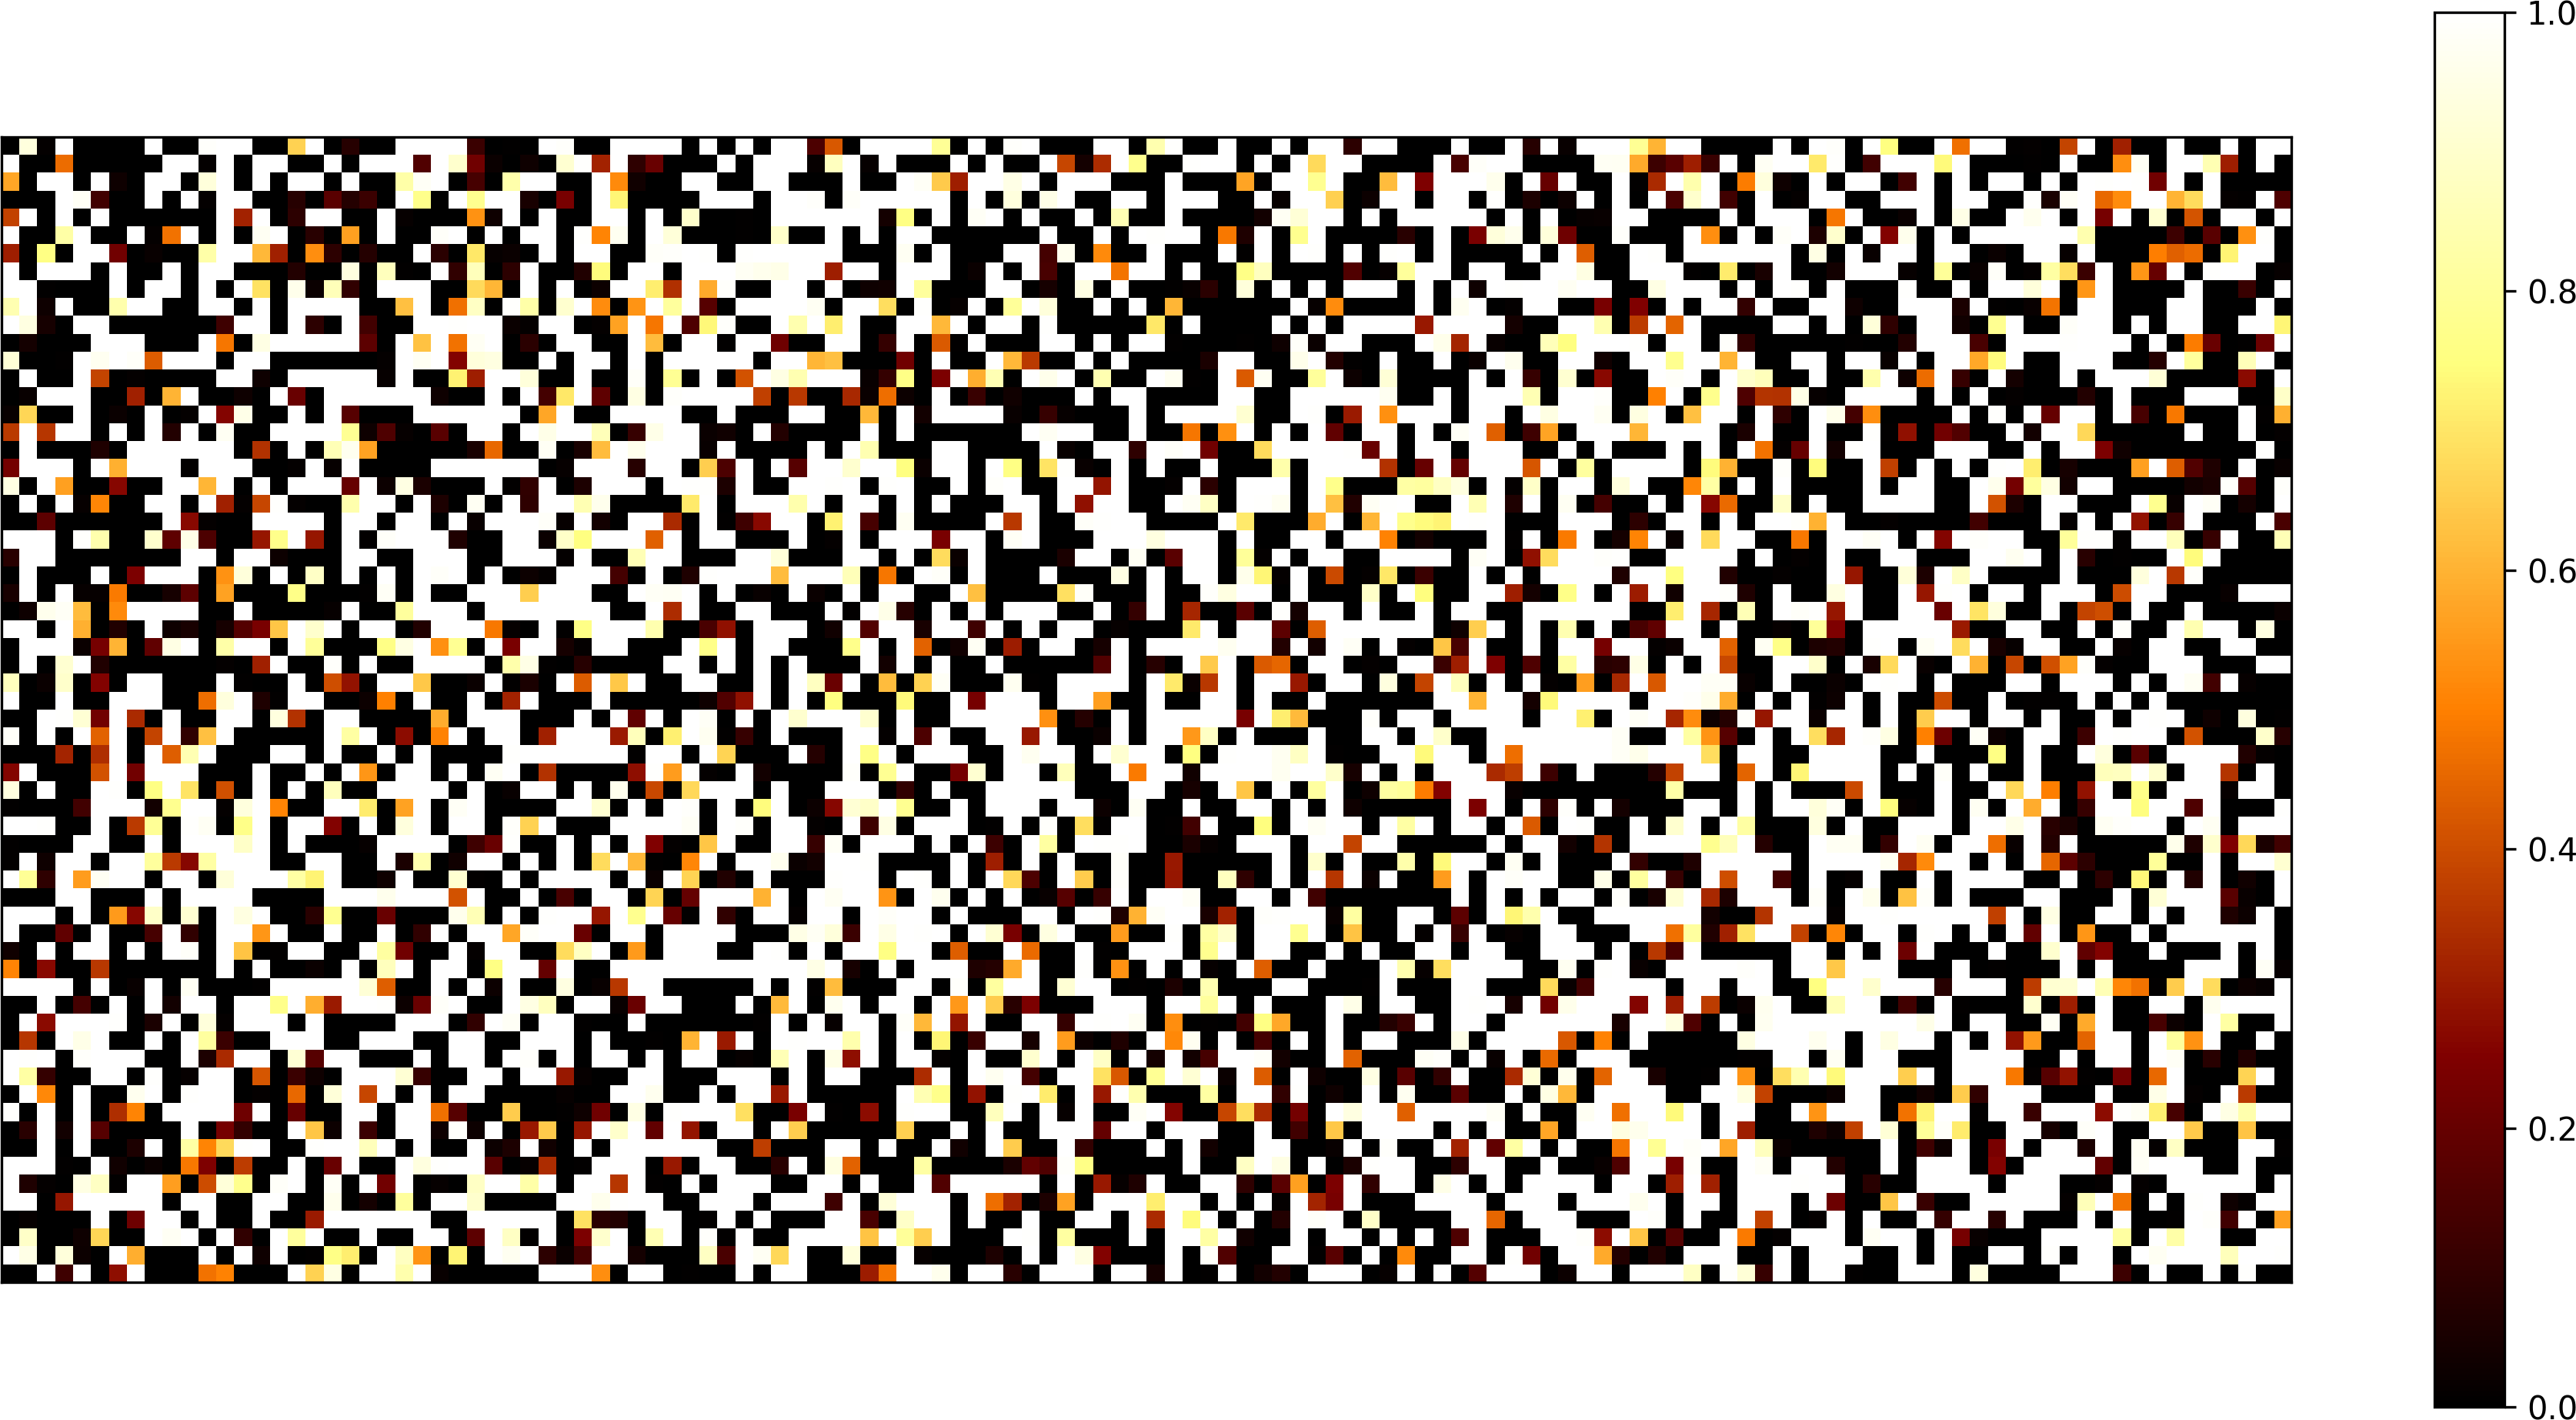
\includegraphics[width=\textwidth]{images/bit_stability.png}
    \caption[Average startup values of individual SRAM cells over 1000 measurements.]{Average startup values of individual SRAM cells over 1000 measurements. White bits are stable `1', black are stable `0' and the rest are unstable bits with varying amounts of instability (according to the color bar on the right). Cells with average value of 0.5 are the least stable. The data was obtained from ESP32 number 12 in 20°C.}
    \label{fig:bit_stability_mask}
\end{figure}

\subsubsection*{Indirect bit preselection}

Indirect preselection runs a test for each bit to identify its stability. For example, stable bit can be identified by the time it takes for it to stabilize its initial state---stable bits stabilize faster than the unstable ones. The test can be performed in the following way.

First, set all the bits to the `0' state. Then, turn off the memory for a short amount of time and look at which bits flipped to the `1' state the fastest. They are the stable `1' bits. Stable `0' bits can be obtained respectively. It has been shown by~\cite{Liu2017} that up to 100\% stable response can be extracted by this method.

\section{SRAM aging}

Normal operation of \gls{sram} memory unavoidably alters its physical properties. These processes can effect the stability of \gls{sram} \gls{puf} and are called silicon aging.

The dominant effect which directly alters the stability of memory cells is called \gls{nbti}. \gls{nbti} is a data-dependent aging effect. If the cell stores a `1' bit, its startup state preference slowly starts to change towards the `0' state. This is the result of a threshold voltage increase on the transistors which are switched on in the currect state, whereas the swithed off transistors are unaffected. This means, that the \gls{sram} \gls{puf} has a natural tendency to become less stable over time if the startup data is left unchanged in memory.\cite{Roelke2018}

Anti-aging techniques, which try to counteract \gls{nbti} and other effects, exist. A simple example is to store an inverse of the startup data after response extraction. However, this is a security risk as leakage of this data would directly reveal the startup memory values. Another solution could be to overwrite the memory with a random string after every power up. This results in less effective anti-aging, but avoids the security risk of a data leak.\cite{Maes2014}



% TODO intrinsicID meli nejaky whitepaper
